%% EAAI submission draft v2 -- elsarticle (author-year / elsarticle-harv).
%% Restructured 2026-08-18 following the organization of arXiv:2505.21574
%% (research-question block in the introduction, prose contributions,
%% run-in related-work paragraphs, a Preliminaries section, and experiment setup as run-in paragraphs).
%% Claims and numbers are unchanged from v1 (main_v1_backup.tex).
%% Compile: pdflatex -> bibtex -> pdflatex x2 (or upload to Overleaf).

\documentclass[preprint,12pt,authoryear]{elsarticle}

\usepackage{graphicx}
\usepackage{booktabs}
\usepackage{amsmath}
\usepackage{amssymb}
\usepackage{url}

\newcommand{\mapm}{mAP\(_{50\text{--}95}\)}

\journal{Engineering Applications of Artificial Intelligence}

\begin{document}

\begin{frontmatter}

\title{Allocation-aware inpainting augmentation for object detection:
the class set, not the per-class weighting, determines where
performance gains occur}

\author[a]{Daehyun Yoo}
\ead{dhyoo970111@gmail.com}
\affiliation[a]{organization={Affiliation to be completed},
                city={},
                country={Republic of Korea}}

\begin{abstract}
Synthetic images produced by diffusion inpainting can enlarge
object-detection training sets at low cost, but a practical question
remains open: given a fixed budget of generated images, which classes
should receive them? The contribution in artificial intelligence is a
controlled answer to this allocation question, obtained with an
allocation-aware background-augmentation framework that protects every
annotated object, regenerates only image backgrounds, and spends a
fixed budget according to an explicit allocation signal --- a frequency-defined tail set versus
a difficulty-defined weak set selected by measured per-class average
precision --- crossed with a within-set weighting (uniform versus
set-specific priority), under fixed budget, class count, generator,
prompts, and rule-based quality verification; the four resulting arms are
evaluated with pre-registered, hash-frozen contrasts, seed-blocked
tests, and multiple-comparison correction. The engineering application
is military aircraft detection in two operationally distinct regimes: a
43-class ground-level natural-view benchmark and a 20-class
satellite-view benchmark, each paired with a compact one-stage detector
and a large pretrained transformer detector. Three results follow.
First, the allocation signal determines where gains occur: each arm
improves the classes it targets (set-by-scope interaction $+0.06$,
corrected $p = 0.017$; replicated at $+0.05$ on the satellite
benchmark), while the within-set uniform-versus-priority contrast is null
in all four comparisons.
Second, every augmentation gain vanishes under the stronger detector,
whose unaugmented baseline exceeds the best augmented compact model.
Third, zero-cost repeat-factor resampling dominates generation on the
deeply imbalanced benchmark but is null on the shallow one, where
inpainting is the only augmentation with significant gains. These
findings yield a three-step engineering rule --- check detector
headroom, probe with free resampling, then generate for the
measured-weakest classes with a uniform split. Code, generated image
pools, and all training artifacts will be released.
\end{abstract}

\begin{keyword}
Data augmentation \sep Diffusion inpainting \sep Object detection \sep
Class imbalance \sep Synthetic data allocation \sep Military aircraft
detection
\end{keyword}

\end{frontmatter}

\section{Introduction}\label{sec:intro}

Object detectors in specialized domains often face uneven data
availability across classes: collecting and annotating representative
images is costly, and the resulting training sets are class-imbalanced.
Military aircraft detection is a useful case study because aircraft
types vary in visual similarity, prevalence, viewpoint, and background.
Diffusion-based synthesis offers one way to expand such training sets,
and generated images have improved classifiers
\citep{azizi2023synthetic, he2023synthetic} and detectors
\citep{suri2024gen2det, feng2024instagen}. For detection, recent work has
primarily improved the generation mechanism through conditioning,
filtering, diversity, and foreground or background editing; background
inpainting can preserve annotated foreground regions while varying their
surroundings \citep{li2024background}. Feedback-guided synthesis and
diffusion curricula have also begun to target underperforming or
underrepresented groups, mainly in classification settings
\citep{hemmat2024feedback, liang2025discl}. What remains unclear for
object detection is whether class-set selection and per-class quota
weighting matter when the total budget, target-set size, generator, and
quality-control protocol are held fixed. We therefore ask two linked
questions:

\begin{quote}\itshape
Given a fixed budget of synthetic images, (i) which classes should
receive it --- the rarest classes or the classes with the lowest
validation performance --- and (ii) once that set is chosen, should the
budget be split uniformly or weighted by priority?
\end{quote}

The two class-selection policies need not agree. Frequency-based
allocation assumes that training frequency is an adequate proxy for the
classes that need additional support. On the natural-view MAD benchmark,
however, the bottom-30\% frequency set and the equally sized weak set
selected by the compact baseline's validation AP averaged over IoU
thresholds 0.50--0.95 are disjoint. Some
rare aircraft types are visually distinctive, whereas several of the
lowest-AP classes occur in the middle or head of the frequency
distribution. In this benchmark, ``help the rare'' and ``help the weak''
are therefore competing allocation policies rather than synonyms. This
separation is an empirical property of the studied data, not an assumed
law relating frequency and difficulty.

We study these choices with an allocation-aware background-augmentation
framework (Figure~\ref{fig:pipeline}). Following the background
inpainting mechanism of \citet{li2024background}, every annotated box is
protected during generation and its source pixels are restored
afterwards. This preserves the geometry and appearance of existing
annotations, although it cannot guarantee that no new, unlabeled object
appears in the regenerated background; we quantify that failure mode
with a detector-based audit and object-gate retraining. The allocation
framework distributes a fixed budget of $B$ images over a target set
chosen by an \emph{allocation signal} (frequency-defined tail vs.\
validation-AP-defined weak) and a \emph{within-set weighting} (uniform
vs.\ set-specific priority). Budget, set size, generator, prompts, and
rule-based verification are fixed, yielding four crossed allocation
arms. The priority score is set-specific, so weighting is compared
within each selected class set rather than interpreted as a single
global main effect. The AI contribution is therefore not a new
diffusion generator, but a controlled framework that separates which
classes receive synthetic data from how the quota is divided among them.
Exploratory experiments on MAD motivated the allocation hypothesis.
Before training the four confirmatory augmentation arms or computing any
confirmatory-arm test-split metric, we time-stamped and hash-froze the
five planned MAD contrasts. The resulting MAD experiment therefore
provides a prospective, seed-level confirmation on the same benchmark,
with inference based on seed-blocked tests and Holm correction. We then
repeated the four-arm design on the separately prepared MAR20 dataset,
whose allocation plan and contrasts were frozen before its untouched
official test split was evaluated, to assess cross-domain replication.

We evaluate the framework on two public military-aircraft benchmarks
with visually distinct imaging regimes: the 43-class natural-view MAD
and the 20-class satellite-view MAR20. Both use a compact one-stage
detector (YOLOv8n) for the complete four-arm design; reduced cells with a
larger pretrained transformer (RT-DETR-L) evaluate RFS and the two
tail-set inpainting arms. Every included arm is trained over three independent
seeds. Three findings emerge. First, on MAD the relative advantage of
the two arm families changes with evaluation scope (set-by-scope
interaction $+0.060$, Holm-adjusted $p = 0.017$), although the pooled
tail- and weak-arm improvements over baseline do not individually survive
Holm correction. MAR20 reproduces the direction and magnitude of the
interaction ($+0.052$), but not confirmatory significance (Holm-adjusted
$p = 0.091$). Across the four within-set comparisons, priority weighting
shows no detectable benefit over a uniform split at the tested budgets;
the confidence intervals do not establish strict equivalence. Second,
in the reduced RT-DETR-L cells, all measured augmentation changes are
near zero or negative relative to the standard-augmentation baseline.
This association is consistent with reduced model headroom, but the
comparison also changes architecture and capacity and does not isolate a
causal mechanism. Third, generation-free RFS strongly outperforms
inpainting on the more imbalanced MAD benchmark but provides no overall
gain on the less imbalanced MAR20 benchmark. Because the datasets differ
in more than imbalance, this contrast motivates a practical hypothesis,
not a general diagnostic law.

Taken together, the study contributes (i) a fixed-budget formulation
that separates class-set selection from within-set weighting, (ii) a
multi-dataset, multi-detector evaluation that identifies where the
observed effects do and do not transfer, and (iii) a configuration-driven
reproducibility package containing allocation plans, generation logs,
per-class metrics, contrast freezes, and weights for 66 primary training
runs. The results suggest a provisional engineering heuristic: establish
a strong standard-augmentation baseline, test generation-free resampling,
and, when additional synthetic data are still warranted, target the
lowest-validation-AP classes with the simpler uniform allocation. Broader
datasets, capacity-matched detectors, and budget-scaling experiments are
needed before this heuristic can be treated as a general rule.

\section{Related work}\label{sec:related}

\subsection{Generative augmentation for detection and instance segmentation}
Building on denoising diffusion models \citep{ho2020ddpm,
rombach2022ldm}, synthetic data has supported image classification
through class-conditional generation \citep{azizi2023synthetic},
zero/few-shot recognition \citep{he2023synthetic}, and language-guided
editing \citep{trabucco2024dafusion, dunlap2023alia}. For detection and
instance segmentation, existing approaches differ chiefly in
\emph{where} synthetic content is introduced and \emph{how} localization
labels are obtained. Instance-composition methods paste real or generated
object cutouts into new scenes: Copy-Paste established the basic recipe
\citep{ghiasi2021copy}; X-Paste scaled it with text-to-image generation
and zero-shot filtering \citep{zhao2023xpaste}; MosaicFusion and DiverGen
extended generated-object augmentation to long-tailed instance
segmentation, with the latter emphasizing category, prompt, and generator
diversity \citep{xie2025mosaicfusion, fan2024divergen}; and SOC recently
scaled object-centric composition while preserving annotation accuracy
across detection, segmentation, and grounding \citep{huang2026soc}.
Full-scene and region-controlled methods
instead synthesize images together with localization cues. InstaGen adds
an instance-level grounding head \citep{feng2024instagen}, Gen2Det couples
grounded scene generation with image- and instance-level filtering
\citep{suri2024gen2det}, ODGEN adapts a layout-conditioned generator to
domain-specific detection data \citep{zhu2024odgen}, AeroGen specializes
layout-conditioned generation for remote sensing
\citep{tang2025aerogen}, and ReCon improves region--text alignment during
sampling without retraining the generator \citep{zhu2025recon}.

Closest to our generation mechanism is background editing:
\citet{li2024background} protect annotated foregrounds and regenerate
their surroundings with Stable Diffusion inpainting, reporting improved
robustness and generalization across their detection benchmarks. We adopt
this mechanism to preserve existing object pixels and bounding-box
geometry; it does not guarantee annotation completeness because a new,
unlabeled object may appear in the regenerated background.

\subsection{Long-tailed detection: resampling and rebalancing}
The long-tail literature --- see \citet{oksuz2021imbalance} and
\citet{zhang2023longtail} for surveys --- conventionally uses class
frequency to characterize imbalance. LVIS introduced a large-vocabulary
benchmark, the rare/common/frequent reporting convention, and
repeat-factor sampling (RFS), a standard image-level resampling scheme
\citep{gupta2019lvis}; instance-aware and exponentially weighted
frequency refinements followed \citep{yaman2023irfs,ahmed2025eirfs}.
Methods developed across long-tailed recognition and detection also
rebalance losses or classifiers, including class-balanced reweighting
\citep{cui2019classbalanced}, equalization and group-softmax losses
\citep{tan2020equalization,li2020bags}, Seesaw loss
\citep{wang2021seesaw}, equalized focal loss for one-stage detectors
\citep{li2022efl}, and decoupled classifier retraining
\citep{kang2020decoupling}. Two implications shape our protocol. First,
evidence from a YOLOv5 study on a constructed long-tailed COCO subset
shows that mosaic and mixup can yield larger gains than sampling- and
loss-based corrections \citep{crasto2024imbalance}. We therefore measure
each primary RFS and inpainting intervention as a \emph{marginal}
addition to the same standard-augmentation baseline. Second, RFS-family
methods use frequency
as the signal for allocating training exposure, but frequency need not
coincide with empirical class difficulty. Accordingly, our protocol uses
RFS as a same-data, generation-free exposure baseline and treats frequency
and empirical difficulty as distinct allocation signals.

\subsection{Allocating and selecting synthetic data}
Model feedback can enter a synthetic-data pipeline at several distinct
stages. In imbalanced classification, \citet{bozorgtabar2019informative}
use Bayesian active-learning scores to select informative cases for
class-aware GAN augmentation, whereas feedback-guided data synthesis uses
one-shot classifier feedback to steer diffusion sampling toward useful
examples \citep{hemmat2024feedback}. DisCL addresses a different decision:
it constructs a spectrum of image-guidance levels and schedules those
levels across training stages for long-tailed and low-quality
classification \citep{liang2025discl}. For long-tailed instance
segmentation, BSGAL instead uses a gradient cache to estimate the
downstream contribution of generated batches and select useful synthetic
examples \citep{zhu2024bsgal}.

Closest to class-wise allocation, MRCA jointly adapts per-class generation
counts, generated-object difficulty, and pasted-object size over multiple
rounds of long-tailed instance-segmentation training
\citep{kim2025mrca}. BSGAL therefore performs model-aware selection from
generated data, whereas MRCA dynamically couples allocation and generation
across training rounds. Our protocol asks a different, deliberately static
question: it freezes every allocation plan before confirmatory training and
compares target-set and within-set quota decisions without adaptive
curation.

\subsection{Aircraft detection in natural and remote-sensing imagery}
Remote-sensing benchmarks span broad object detection, as in DOTA
\citep{xia2018dota} and DIOR \citep{li2020dior}, and fine-grained
recognition, as in FAIR1M \citep{sun2022fair1m}. Military-aircraft
recognition has a dedicated large public benchmark in MAR20, which
contains 3{,}842 satellite images, 20 aircraft types, and both horizontal
and oriented box annotations \citep{yu2023mar20}. Architecture-centered
work includes the one-stage FGA-YOLO, evaluated on MAR20 and FAIR1M
\citep{wu2025fga}; related work in this journal addresses generic UAV
small-object detection through multi-scale attention
\citep{song2024small}.

Aircraft-specific work has also compared augmentation mechanisms.
\citet{shermaine2025compositing} evaluate classical augmentation, image
compositing, Stable Diffusion XL, and ControlNet with YOLOv8 on a custom
dataset of commercial and military aircraft. The public web-image MAD
dataset and satellite-view MAR20 benchmark let us examine allocation in
two distinct imaging regimes, with selected policies additionally tested
across detector families.

\subsection{Positioning of this study}
Across these strands, prior work separately improves generation,
rebalancing, model-guided selection, and aircraft-specific augmentation.
It has not directly compared equally sized frequency- and
validation-AP-defined target sets while varying quotas within each set
under a fixed detection pipeline and generation budget. We address that
controlled policy comparison using four frozen arms: each target set is
paired with uniform quotas and its own pre-specified priority rule. Our
inference therefore concerns the two within-set uniform-versus-priority
contrasts and the set-by-scope interaction, not a universal weighting
main effect or a universally superior allocation signal.

\section{Preliminaries}\label{sec:prelim}

\paragraph{Problem formulation}
Let $\mathcal{C}$ denote the class set of a detection dataset with
train/val/test splits, and let $B \in \mathbb{N}$ be a fixed budget of
synthetic images. An \emph{allocation plan} is a pair $(S, q)$ of a
target set $S \subseteq \mathcal{C}$ with $|S| = K$ and a quota vector
$q \in \mathbb{N}^{S}$ with $\sum_{c \in S} q_c = B$, assigning each
target class $c$ a number $q_c$ of synthetic images generated from
training images that contain $c$. We decompose the plan into two
decisions: the \emph{allocation signal} that selects $S$, and the
\emph{within-set quota rule} that shapes $q$ given $S$. An
\emph{augmentation arm} is the training condition obtained by adding the
$B$ generated images of one plan to the training split; validation and
test splits are never modified.

\paragraph{Evaluation scopes and metric}
Performance is reported as mean average precision over
intersection-over-union thresholds 0.50--0.95 (\mapm) on the test
split. For a class subset $G \subseteq \mathcal{C}$ (a \emph{scope}),
the macro score is the unweighted mean of per-class AP over $G$. We
evaluate three scopes --- \emph{all} ($G = \mathcal{C}$), the
frequency-defined \emph{tail}, and the AP-defined \emph{weak} set ---
and always report gains $\Delta$ relative to the same-cell augmented
baseline.

\paragraph{Resampling baseline}
Repeat-factor sampling \citep[RFS;][]{gupta2019lvis} is the zero-cost
resampling reference: with $f(c)$ the fraction of training images
containing class $c$, each image $I$ is duplicated according to
$r(I) = \max_{c \in I} r(c)$, where
$r(c) = \max\!\bigl(1, \sqrt{t/f(c)}\bigr)$ with $t = 0.1$, materialized
at the dataset level. Because RFS re-exposes existing pixels only, it
serves both as a strong baseline and as a probe that separates
exposure-driven from variation-driven gains (Section~\ref{sec:r3}).

\section{Allocation-aware background augmentation}\label{sec:framework}

We instantiate the allocation problem of Section~\ref{sec:prelim}
with a generation mechanism that exactly preserves source-object pixels,
boxes, and labels, a
deterministic allocator, rule-based verification, and a pre-registered
evaluation protocol (Figure~\ref{fig:pipeline}).

\begin{figure}[t]
\centering

\includegraphics[width=\linewidth]{figures/fig1_pipeline_design.pdf}
\caption{Framework overview. (a)~Generation pipeline: all annotated
boxes in a source image are geometrically protected; diffusion
inpainting regenerates only the background; outputs must pass
rule-based verification (with budget refill) before insertion into the
training split. Budget $B$, class count $K$, generator, prompts, and
verification are held fixed across arms. (b)~The four-arm crossed
allocation design: each class set (frequency-defined tail or AP-defined
weak) is paired with uniform quotas and a set-specific priority rule.}
\label{fig:pipeline}
\end{figure}

\subsection{Allocation signals and within-set quota rules}\label{sec:alloc}

We instantiate two allocation signals and, within each selected set,
compare uniform quotas with a set-specific priority rule, yielding four
crossed augmentation arms:
\begin{itemize}
\item \textbf{Tail set (frequency signal).} The bottom 30\% of classes
  by training instance count --- the conventional long-tail
  prescription.
\item \textbf{Weak set (difficulty signal).} The $K$ classes with the
  lowest baseline per-class AP, measured on the validation split by the
  \texttt{basic\_aug} baseline detector and averaged over its training
  seeds. $K$ is fixed to the tail-set size so that set identity, not set
  size, is the manipulated variable.
\item \textbf{Uniform allocation} splits $B$ equally across the $K$
  classes.
\item \textbf{Priority allocation} distributes $B$ proportionally to a
  priority score: for the tail set, a convex combination of rarity and
  measured weakness (weight 0.6 toward rarity); for the weak set,
  measured weakness alone.
\end{itemize}
Because the two priority scores are not identical, uniform versus
priority is evaluated within each target set; we do not estimate a common
weighting main effect across sets.
Quotas are computed by a deterministic capped largest-remainder
allocator: each class first receives a minimum quota, the remainder is
apportioned according to the selected quota rule under per-class caps, and
fractional leftovers go to the largest remainders with index-ordered tie
breaking. The allocator guarantees that every arm spends exactly $B$
images on exactly $K$ classes, so budget can never confound the
comparison. Empirically, the two sets are disjoint on the natural-view
benchmark and overlap only marginally on the satellite-view benchmark
(Section~\ref{sec:exp}) --- frequency and measured difficulty select
genuinely different classes here (Section~\ref{sec:r1}), which is what
renders the crossed comparison informative.

\subsection{Source-object-preserving background generation}\label{sec:generation}

Synthetic images are produced with Stable Diffusion inpainting
\citep[\texttt{runwayml/stable-diffusion-inpainting};][]{rombach2022ldm}
at 16-bit floating-point precision, 20 denoising steps, guidance scale
7.5, and strength 0.85, at $512\times512$ working resolution and resized
back to the source resolution. For each source image we build a mask
that \emph{protects} all annotated boxes with a 10\% padding margin and
a blurred boundary band, so that diffusion may alter only the
background. Scene prompts are dataset-specific (five natural-view
aviation prompts for MAD; five top-down aerodrome prompts for MAR20), as
are the negative prompts, which suppress --- among other artifacts ---
the generation of new aircraft. After generation, the protected regions
are pasted back from the source pixels, making source-object appearance
and source bounding boxes exact copies; their labels are copied
unchanged. This preserves the source annotations exactly but does not
guarantee annotation completeness for a new object introduced in the
regenerated background.
Generation is fully deterministic given the plan: each output is a
function of the source image, the prompt rotation, and a derived
per-image seed, which enables byte-identical regeneration and safe reuse
across experiments (examples in Figure~\ref{fig:examples}; additional
source/generated pairs in \ref{app:gen}).

\subsection{Rule-based quality verification and budget refill}\label{sec:verify}

Source images must first offer enough editable background for inpainting
to be meaningful (protected regions covering no more than 95\% of the
frame); sources failing this pre-check are excluded before generation.
Every generated image must then pass two quantitative checks: (i)~the
background changed substantially (mean absolute pixel difference $\geq
10$ gray levels outside the boxes), and (ii)~the protected interiors did
not change beyond a compression-noise tolerance ($\leq 5$ gray levels).
Failed generations are retried and, if still failing, replaced from
alternative sources within a bounded attempt budget until the class
quota is met, so all arms reach the same \emph{realized} budget. A run
aborts if more than half of all attempts fail, flagging generator
malfunction. As an additional audit --- reported as a robustness check,
not a filter --- a detector-based scan counts \emph{hallucinated}
objects that diffusion occasionally paints into backgrounds, and an
object-level gate variant retrains the arms with all affected images
removed (Section~\ref{sec:robust}).

\subsection{Pre-registered statistical protocol}\label{sec:stats}

We separate planning from evaluation. All plan-forming measurements
(weak set selection, priority scores) use the validation split only; the
test split is reserved for final reporting, and no plan or
hyperparameter was revised after observing test metrics. For the
four-arm cells, five contrasts were specified and frozen --- with
a content hash and timestamp --- before any test-split metric existed:
(1)~tail arms vs.\ baseline on the tail scope, (2)~weak arms vs.\
baseline on the weak scope, (3)~the set-by-scope interaction,
(4--5)~weighted vs.\ uniform within each set. Contrasts are evaluated on
per-seed macro AP with seed-blocked paired $t$-tests ($n = 3$
independent training seeds) and Holm correction \citep{holm1979simple}
within each cell's five-contrast family; all tests are two-sided at
$\alpha = 0.05$. Wilcoxon signed-rank tests on seed-averaged per-class
AP provide secondary, distribution-free evidence.

\section{Experiments}\label{sec:exp}

The engineering application is military aircraft detection in two
operationally distinct imaging regimes --- ground-level natural views
and satellite views --- a setting where per-class data collection is
expensive and class imbalance is unavoidable, making augmentation budget
decisions a practical engineering concern. Both benchmarks are publicly
available, supporting replication of every result.

\subsection{Datasets}
\textbf{MAD} \citep[Military Aircraft Detection, natural side/ground
views; public;][]{rookieengg2023mad} contains 11{,}788 images
(9{,}430/1{,}179/1{,}179 train/val/test) with 18{,}832 boxes over 43
aircraft types; the train-split imbalance ratio is 10.5. \textbf{MAR20}
\citep[Military Aircraft Recognition dataset, satellite view, horizontal
boxes; public;][]{yu2023mar20} provides an official test split of
2{,}511 images, which we preserve untouched for final reporting; the
official 1{,}331 training images are split 80/20 into train/val with
class-stratified sampling. MAR20's 20-class distribution is markedly
shallower than MAD's, which Section~\ref{sec:r3} exploits as a natural
contrast in imbalance structure. The tail set is a property of the
dataset; the weak set is derived from each detector's own baseline
(Section~\ref{sec:alloc}) and is therefore cell-specific. On MAD the two
sets contain 13 classes each and are disjoint for both detectors; on
MAR20 they contain 6 classes each, overlapping in one class for the
compact detector and two for the transformer.

\subsection{Detectors and training}
We use two detectors spanning an order of magnitude in capacity:
YOLOv8n, a compact one-stage detector of the You-Only-Look-Once (YOLO)
family (3.2M parameters), and RT-DETR-L, the large variant of the
Real-Time Detection Transformer \citep[32M parameters;][]{zhao2024rtdetr}.
Both are initialized from checkpoints pretrained on the Common Objects
in Context (COCO) benchmark \citep{lin2014coco}, so the cells differ in capacity and
architecture family, not in pretraining corpus. Both are trained at
$640\times640$ for 50 epochs with early stopping (patience 15) under
identical schedules across arms within the Ultralytics framework
\citep{jocher2023ultralytics}; the batch size is fixed to 8 for
RT-DETR-L and set automatically for YOLOv8n, with all remaining
hyperparameters at framework defaults. \texttt{real\_only} (framework
augmentation disabled) is a reference lower bound and
\texttt{basic\_aug} (default photometric/geometric augmentation) is the
baseline all gains are measured against. Every arm--cell combination is
trained with three independent seeds; all statistics aggregate over
seeds as described in Section~\ref{sec:stats}.

\subsection{Cells and budgets}
Table~\ref{tab:cells} summarizes the four dataset $\times$ detector
cells. The YOLOv8n cells run the complete four-arm crossed design plus
baselines; the RT-DETR-L cells run a reduced design (baseline, RFS, and
the two tail-set arms) intended to test whether gains transfer to a
stronger detector rather than to re-estimate the interaction. The
uniform arm's pool depends only on the dataset and is shared across the
detector cells; the weighted arm's difficulty component is recomputed
from each detector's own baseline validation AP, so its allocation is
detector-specific. Budgets scale with dataset size: $B = 1{,}000$
($K = 13$, per-class quota 5--200) for MAD and $B = 500$ ($K = 6$, quota
5--100) for MAR20. Realized budgets equal planned budgets in all cells
(verification failure rates: $\leq 21\%$ of attempts on MAD, 0.6\% on
MAR20, absorbed by the refill mechanism of Section~\ref{sec:verify}).

\subsection{Reproducibility}
Generation is seed-deterministic given a plan
(Section~\ref{sec:generation}); plans, generation logs, verification
reports, contrast freezes (with content hashes), per-class metrics, and
trained weights for all 66 primary training runs --- plus the
object-gate retrainings of Section~\ref{sec:robust} --- are archived,
and the full pipeline, from dataset normalization to the statistical
reports, runs from configuration files without manual intervention.
Prompts, class memberships, realized per-class quotas, and measured
compute are listed in \ref{app:gen}. Code and artifacts will be
released upon publication.

\begin{table}[t]
\centering
\caption{Experimental cells. All cells share the generation,
verification, and statistical protocol.}
\label{tab:cells}
\begin{tabular}{llll}
\toprule
Dataset & Detector & Arms & Budget $B$\,/\,$K$ \\
\midrule
MAD   & YOLOv8n   & full $2\times2$ + RFS + baselines & 1{,}000\,/\,13 \\
MAD   & RT-DETR-L & reduced (tail-set arms + RFS)     & 1{,}000\,/\,13 \\
MAR20 & YOLOv8n   & full $2\times2$ + RFS + baselines & 500\,/\,6 \\
MAR20 & RT-DETR-L & reduced (tail-set arms + RFS)     & 500\,/\,6 \\
\bottomrule
\end{tabular}
\end{table}

\subsection{The allocation signal determines where gains occur}\label{sec:r1}

\paragraph{Frequency and difficulty select different classes}
On MAD, per-class training-instance count and baseline test AP correlate
\emph{negatively} (\mapm{} basis; Pearson $r = -0.375$, $p = 0.013$;
Spearman $\rho = -0.408$, $p = 0.007$; Figure~\ref{fig:freqap}). In
AP\(_{50}\) terms, the rarest class (YF-23, 97 training instances)
attains the highest score (0.93), whereas the weakest classes (Rafale
0.31, F-14 0.37) sit in the medium and head frequency ranges.
Empirically, the frequency-defined tail set and the AP-defined weak set
are disjoint on MAD (0/13 overlap) and overlap in a single class on
MAR20 for the compact detector. This is the premise that makes the
$2\times2$ allocation design informative: if frequency were a good
proxy for difficulty, the two signals would select the same classes and
could not be dissociated.

\begin{figure}[t]
\centering

\includegraphics[width=0.85\linewidth]{figures/fig2_freq_vs_ap.pdf}
\caption{Frequency is a poor proxy for difficulty on MAD. Per-class
baseline test \mapm{} (three-seed mean) against training instance count
(log scale). The frequency-defined tail set (blue) and the AP-defined
weak set (orange) are disjoint; the rarest class (YF-23) is the easiest,
while the weakest classes (Rafale, F-14) sit at medium-to-head
frequency.}
\label{fig:freqap}
\end{figure}

\paragraph{Gains land on the targeted set (MAD, confirmatory)}
Figure~\ref{fig:dissoc} (left) shows the result on MAD with YOLOv8n as a
double dissociation: each set family improves its own target scope
substantially more than the other family does, and vice versa. Averaged
over seeds, the two tail-set arms improved the tail scope by $+0.061$
over baseline while improving the weak scope by only $+0.019$; the two
weak-set arms showed the mirrored pattern ($+0.040$ on weak, $+0.022$ on
tail). The pre-registered set-by-scope interaction --- the
difference-in-differences of the two set families across the two scopes
--- was $+0.0598$ (95\% CI $[0.045, 0.075]$, Holm-adjusted
$p = 0.017$), with all three seeds showing the same direction. At the
class level, gains were broad rather than concentrated: 11 of 13 tail
classes improved under the tail-uniform arm (largest: Tu-95 $+0.169$,
MiG-31 $+0.101$), and 11 of 13 weak classes improved under the
weak-uniform arm (largest: Tornado $+0.123$, Rafale $+0.086$ --- the
weakest class in the dataset); the full sorted distributions are shown
in Figure~\ref{fig:perclass} and tabulated in \ref{app:perclass}.

\begin{figure}[t]
\centering
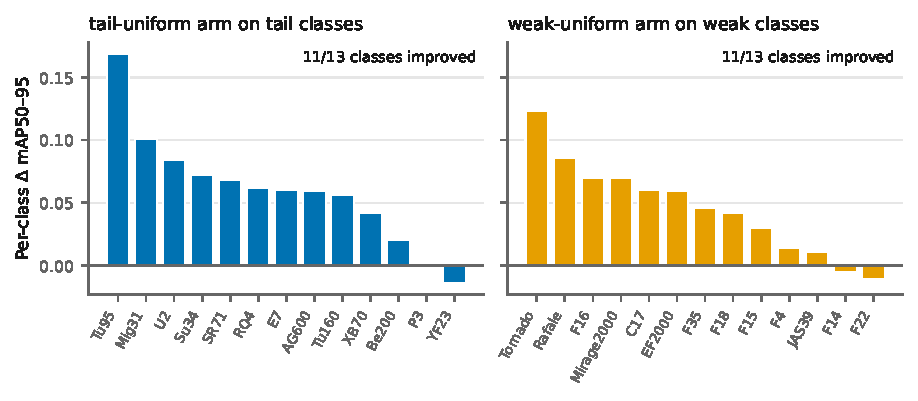
\includegraphics[width=\linewidth]{figures/fig6_perclass_delta.pdf}
\caption{Per-class gains are broad rather than concentrated. Sorted
per-class $\Delta$ \mapm{} (3-seed means) of the two uniform arms on
their targeted MAD classes; 11 of 13 classes improve in each set.}
\label{fig:perclass}
\end{figure}

\begin{figure}[t]
\centering

\includegraphics[width=\linewidth]{figures/fig3_dissociation.pdf}
\caption{The allocation signal determines where gains occur. $\Delta$
\mapm{} versus the same-cell baseline for the four inpainting arms on
the tail scope (blue) and weak scope (orange); black-edged bars mark
each arm's targeted scope; error bars span $\pm 1$ standard deviation
over three seeds. Left: MAD (confirmatory; interaction Holm-adjusted
$p = 0.017$). Right: MAR20 (replication of the effect size;
Section~\ref{sec:r1}).}
\label{fig:dissoc}
\end{figure}

\paragraph{The dissociation replicates in the satellite domain (MAR20)}
Figure~\ref{fig:dissoc} (right) shows the same analysis for MAR20 with
YOLOv8n. The interaction estimate was $+0.0523$ (95\% CI
$[0.021, 0.083]$; positive in all three seeds), which lies inside the
95\% CI of the MAD estimate; the tail-targeted arm again gained most on
the tail scope (selective: $+0.044$; class-level Wilcoxon $p = 0.031$,
the smallest attainable value at $n = 6$) and the weak-targeted arms
most on the weak scope ($+0.030$ to $+0.034$). Because the MAR20 scopes
contain only six classes each, the seed-blocked tests are underpowered
and the interaction does not survive Holm correction (unadjusted
$p = 0.018$, Holm-adjusted $p = 0.091$); we therefore report MAR20 as an
independent replication of the effect size rather than a second
confirmatory result.

\paragraph{Within-set weighting shows no benefit}
In contrast to the choice of class set, \emph{how} the fixed budget is
divided inside the chosen set showed no evidence of benefit in any
condition: the weighted-versus-uniform contrasts were null in all four
pre-registered comparisons, with estimates centred near zero ($+0.002$,
$p = 0.81$ and $-0.012$, $p = 0.17$ on MAD; $+0.014$, $p = 0.11$ and
$+0.004$, $p = 0.52$ on MAR20; Table~\ref{tab:contrasts}). The CIs do
not exclude small effects in either direction, so we do not claim strict
equivalence; what the data rule out is a within-set weighting benefit
comparable to the set-choice effect. Given that the uniform and weighted
arms shared the same class sets, generator, prompts, quality
verification, and budget, we conclude that at the budgets studied the
allocation \emph{signal} (which classes) --- not the allocation
\emph{shape} (how many per class) --- is the operative variable.

\paragraph{Targeted gains come with a smaller global spillover}
Augmenting one set also produced consistent but smaller gains outside
it: on MAD the tail-uniform arm improved the weak scope by $+0.031$
(class-level $p = 0.002$), and on MAR20 the cross-set gains ranged from
$+0.004$ to $+0.013$. Background inpainting therefore appears to combine
a set-specific targeting component with a smaller domain-wide component,
consistent with the recall-oriented mechanism discussed in
Section~\ref{sec:discussion}.

\subsection{A strong pretrained detector removes all augmentation gains}\label{sec:r2}

Replacing the compact detector with RT-DETR-L raised the baseline from
0.575 to 0.869 on MAD and from 0.572 to 0.697 on MAR20 --- and
eliminated every augmentation effect we measured
(Figure~\ref{fig:condmap}, Table~\ref{tab:master}). On MAD, all deltas
were zero to negative: uniform $-0.004$, selective $-0.001$, and RFS
$-0.016$; the pooled inpainting-versus-baseline contrast on the tail
scope was $-0.008$ ($p = 0.36$). On MAR20 the pattern repeated (uniform
$-0.007$, selective $-0.005$, RFS $+0.003$; pooled tail contrast
$+0.004$, $p = 0.72$). Notably, the strong detector's \emph{baseline}
already exceeded the best augmented YOLOv8n result by a wide margin
(0.869 vs.\ 0.661 on MAD).

Two observations follow. First, augmentation gains in this study are
conditional on detector headroom: once a model retains little headroom
on the dataset, neither resampling nor generative augmentation adds
measurable value, and the largest single lever is the detector upgrade
itself (a cross-cell comparison; Section~\ref{sec:rules}). Second, the
only consistently \emph{negative} delta under the strong detector was
RFS on MAD ($-0.016$ on all three scopes), suggesting that increasing
duplicate exposure can be mildly harmful when capacity and pretraining
already suffice; we report this as an observation without claiming a
mechanism. Because the RT-DETR-L cells implemented a reduced design
(baseline, RFS, and the two tail-set arms only), no interaction test is
available there; the ``vanishing gains'' claim rests on the near-zero
deltas of all measured arms.

\begin{figure}[t]
\centering

\includegraphics[width=0.9\linewidth]{figures/fig4_condition_map.pdf}
\caption{Condition map across the four cells. Best augmentation
$\Delta$ \mapm{} (all scope) against the unaugmented baseline of each
cell; triangles denote repeat-factor sampling, circles the best
inpainting arm; color denotes the dataset. Gains shrink to zero under
the high-baseline RT-DETR-L cells (right), and resampling and inpainting
exchange ranks between MAD and MAR20 (left).}
\label{fig:condmap}
\end{figure}

\subsection{Resampling effectiveness depends on the imbalance structure}\label{sec:r3}

Repeat-factor sampling --- the zero-cost resampling baseline that
dominated every diffusion arm on MAD ($+0.086$ all, $+0.098$ tail,
$+0.117$ weak; class-level $p \leq 2\times10^{-4}$) --- transferred
poorly to MAR20. With the same detector and protocol, RFS on MAR20
yielded $+0.003$ (all), $+0.016$ (tail), and $-0.011$ (weak;
class-level $p = 0.031$) --- the only statistically significant negative
augmentation effect we observed under YOLOv8n. MAD is deeply imbalanced
across 43 classes (max/min instance ratio 10.5), so re-exposing
rare-class images carries additional training signal; MAR20's 20-class
distribution is comparatively shallow, and additional exposure of
already-seen images adds little, while inpainting --- which injects
genuinely new background variation --- remains effective
(Section~\ref{sec:r1}). On MAR20, inpainting was in fact the only
augmentation with statistically significant gains. The practical
implication is developed in Section~\ref{sec:discussion}: RFS is a cheap
first attempt rather than a universal winner, and its failure is
diagnostic of a regime where generative augmentation is worth its cost.

\subsection{Robustness checks}\label{sec:robust}

\paragraph{Generation quality does not explain the dissociation}
The three originally generated MAD pools passed rule-based quality
verification at similar rates (79--82\%), and the fourth pool reached
its quota under the same criteria; per-pool Fr\'{e}chet inception
distance \citep[FID;][]{heusel2017fid} and CLIP-based image--text
similarity scores \citep{radford2021clip} were comparable, with the
\emph{worst}-FID pool (weakness) producing the significant weak-scope
gain --- quality differences cannot account for where gains landed. On
MAR20 the verification failure rate was 0.6\%, and all four pools
reached the full 500-image budget.

\paragraph{Hallucinated objects do not drive the RFS gap on MAD}
A detector-based audit found unlabeled aircraft hallucinated into 10.2\%
of MAD synthetic backgrounds (see Figure~\ref{fig:examples}, top row).
Removing all affected images with an object-level gate and retraining
the three original diffusion arms changed their all-scope performance by
at most $|\Delta| \leq 0.017$ (all nine gated-versus-ungated comparisons
non-significant, $p = 0.11$--$0.97$), while the RFS advantage persisted
essentially unchanged ($\Delta = -0.055$ to $-0.067$ versus RFS,
$p < 10^{-4}$). A full-corpus gate scan removed 332 of the 3{,}000
images (11.1\%; 845 hallucinated objects), consistent with the
audit-sample estimate; per-pool statistics and the gated retraining
results are given in \ref{app:audit}. Label noise from generation
artifacts therefore explains neither the dissociation nor the
resampling gap.

\begin{figure}[t]
\centering

\includegraphics[width=0.8\linewidth]{figures/fig5_generation_examples.pdf}
\caption{Generation examples (source, protection mask, output; mask
black = protected). Rows: two MAD and two MAR20 cases spanning
formation, airshow, apron, and airbase scenes. The top row also
illustrates the hallucination failure mode quantified in
Section~\ref{sec:robust} --- diffusion has painted additional, unlabeled
aircraft into the regenerated sky --- which motivates the detector-based
audit and the object-gate robustness check.}
\label{fig:examples}
\end{figure}

\begin{table}[t]
\centering
\caption{Master results: $\Delta$ \mapm{} versus the same-cell
\texttt{basic\_aug} baseline (mean over three seeds; baseline rows show
absolute mAP $\pm$ SD). Bold marks the scope targeted by each arm;
scopes are cell-specific (Section~\ref{sec:exp}).}
\label{tab:master}
\small
\begin{tabular}{llrrr}
\toprule
Dataset $\times$ detector & Arm & all & tail & weak \\
\midrule
MAD $\times$ YOLOv8n
  & basic\_aug    & $0.575\pm0.007$ & $0.620\pm0.009$ & $0.456\pm0.030$ \\
  & RFS           & $+0.086$ & $+0.098$ & $+0.117$ \\
  & tail-uniform  & $+0.031$ & $\mathbf{+0.060}$ & $+0.031$ \\
  & tail-weighted & $+0.023$ & $\mathbf{+0.062}$ & $+0.007$ \\
  & weak-uniform  & $+0.016$ & $+0.014$ & $\mathbf{+0.046}$ \\
  & weak-weighted & $+0.020$ & $+0.030$ & $\mathbf{+0.034}$ \\
\midrule
MAD $\times$ RT-DETR-L
  & basic\_aug    & $0.869\pm0.006$ & $0.889\pm0.008$ & $0.842\pm0.012$ \\
  & RFS           & $-0.016$ & $-0.010$ & $-0.016$ \\
  & tail-uniform  & $-0.004$ & $\mathbf{-0.013}$ & $-0.006$ \\
  & tail-weighted & $-0.001$ & $\mathbf{-0.004}$ & $+0.003$ \\
\midrule
MAR20 $\times$ YOLOv8n
  & basic\_aug    & $0.572\pm0.005$ & $0.532\pm0.013$ & $0.467\pm0.017$ \\
  & RFS           & $+0.003$ & $+0.016$ & $-0.011$ \\
  & tail-uniform  & $+0.010$ & $\mathbf{+0.030}$ & $+0.013$ \\
  & tail-weighted & $+0.012$ & $\mathbf{+0.044}$ & $+0.008$ \\
  & weak-uniform  & $+0.004$ & $+0.008$ & $\mathbf{+0.030}$ \\
  & weak-weighted & $+0.003$ & $+0.004$ & $\mathbf{+0.034}$ \\
\midrule
MAR20 $\times$ RT-DETR-L
  & basic\_aug    & $0.697\pm0.001$ & $0.676\pm0.007$ & $0.611\pm0.010$ \\
  & RFS           & $+0.003$ & $+0.013$ & $0.000$ \\
  & tail-uniform  & $-0.007$ & $\mathbf{+0.007}$ & $-0.009$ \\
  & tail-weighted & $-0.005$ & $\mathbf{0.000}$  & $-0.007$ \\
\bottomrule
\end{tabular}
\end{table}

\begin{table}[t]
\centering
\caption{Pre-registered contrasts (seed-blocked paired $t$, $n = 3$
seeds; Holm correction within each cell's five-contrast family). Both
four-arm cells use YOLOv8n (Section~\ref{sec:exp}).}
\label{tab:contrasts}
\small
\begin{tabular}{llrrrr}
\toprule
Dataset & Contrast & Estimate & 95\% CI & $p$ & Holm $p$ \\
\midrule
MAD & Tail arms vs.\ baseline (tail scope)  & $+0.061$ & $[+0.026, +0.096]$ & 0.017 & 0.069 \\
MAD & Weak arms vs.\ baseline (weak scope)  & $+0.040$ & $[-0.021, +0.100]$ & 0.106 & 0.317 \\
MAD & \textbf{Set $\times$ scope interaction} & $\mathbf{+0.060}$ & $\mathbf{[+0.045, +0.075]}$ & \textbf{0.003} & \textbf{0.017} \\
MAD & Weighted vs.\ uniform (tail set)    & $+0.002$ & $[-0.031, +0.035]$ & 0.808 & 0.808 \\
MAD & Weighted vs.\ uniform (weak set)    & $-0.012$ & $[-0.036, +0.013]$ & 0.172 & 0.345 \\
\midrule
MAR20 & Tail arms vs.\ baseline (tail scope)  & $+0.037$ & $[+0.015, +0.058]$ & 0.018 & 0.091 \\
MAR20 & Weak arms vs.\ baseline (weak scope)  & $+0.032$ & $[-0.024, +0.087]$ & 0.133 & 0.336 \\
MAR20 & Set $\times$ scope interaction & $+0.052$ & $[+0.021, +0.083]$ & 0.018 & 0.091 \\
MAR20 & Weighted vs.\ uniform (tail set)    & $+0.014$ & $[-0.008, +0.035]$ & 0.112 & 0.336 \\
MAR20 & Weighted vs.\ uniform (weak set)    & $+0.004$ & $[-0.019, +0.027]$ & 0.519 & 0.519 \\
\bottomrule
\end{tabular}
\end{table}

\section{Discussion}\label{sec:discussion}

\subsection{Engineering guidance: a three-step decision rule}\label{sec:rules}

Read together, the four cells yield an actionable procedure for
practitioners who must decide whether --- and how --- to spend a
synthetic-data budget on a detection system.

\paragraph{Step 1: assess detector headroom before investing in
augmentation}
The largest single improvement observed in this study came not from any
data intervention but from replacing the detector: the pretrained
transformer's \emph{unaugmented} baseline exceeded the best augmented
result of the compact detector by 0.21 \mapm{} on MAD (0.869 vs.\
0.661), and once the stronger detector was in place, every augmentation
we measured was ineffective and resampling was mildly harmful
(Section~\ref{sec:r2}). We stress that this is a cross-cell engineering
observation rather than a randomized comparison --- the two detectors
differ simultaneously in capacity and architecture family (both are
initialized from COCO-pretrained weights) --- but its practical reading
held in every condition we tested: when deployment constraints permit a
stronger pretrained detector, the model upgrade dominated every
augmentation decision we evaluated. Data-side interventions become
worth considering primarily where a compact detector is mandated, for
example by edge-compute budgets, and the model therefore retains
visible headroom.

\paragraph{Step 2: use free resampling as a first attempt --- and as a
diagnostic}
Repeat-factor sampling requires no generation compute and, on the deeply
imbalanced MAD (imbalance ratio 10.5), outperformed every diffusion arm
on every scope (Section~\ref{sec:r3}). Its benefit did not transfer to
the shallowly imbalanced MAR20, where it was null overall and negative
on the weak scope. Because resampling can only re-expose existing
images, it helps precisely when under-exposure of rare classes is the
binding constraint; its failure therefore signals that the constraint
lies elsewhere --- in the diversity of the training distribution rather
than in exposure frequency --- which is the regime where injecting
genuinely new variation through generation remains the available lever.
In practice, RFS functions as a low-cost probe: run it first, keep it if
it helps, and read a null result as evidence that a generative budget
may be worth its price.

\paragraph{Step 3: when generating, select the class set by measured
difficulty; per-class quota tuning is unnecessary}
The interaction result (Section~\ref{sec:r1}) shows that the allocation
signal determines where gains occur, whereas the within-set weighting
axis was null in all four pre-registered comparisons. This simplifies
deployment considerably: the only consequential choice is which classes
to target. Frequency is the conventional default for that choice, but it
is a poor one whenever frequency and difficulty decouple, as they do
here ($r = -0.375$). If the operational goal is to lift worst-case class
performance, the per-class validation AP of the current baseline ---
available at no additional cost in any trained system --- is the direct
signal, and targeting the lowest-AP classes aligns the expected gains
with that goal; within the chosen set, a uniform split of the budget
suffices. The compute cost is moderate: generating and verifying one
thousand 512-pixel background variants took a few GPU-hours on a single
mid-range accelerator in our experiments, of the same order as one
detector training run at this scale.

\subsection{Why background inpainting behaves this way}

Three observations jointly constrain the interpretation. First, the
compact detector's dominant error mode on MAD is missed detection:
baseline recall (0.52--0.59) trails precision (0.62--0.71), and the
largest off-diagonal mass in the confusion structure assigns true
objects to background (Figure~\ref{fig:confusion} in \ref{app:audit}). Second, gains concentrate on the targeted set yet
consistently spill over, attenuated, to non-targeted classes
(Section~\ref{sec:r1}). Third, all gains vanish under the
higher-capacity pretrained detector (Section~\ref{sec:r2}). These
observations are consistent with a single account: background inpainting
counteracts \emph{background overfitting}. Re-rendering the surroundings
of a geometrically protected object weakens context cues spuriously
correlated with class identity, forcing the detector to rely on object
appearance and thereby recovering missed detections --- most strongly
for classes whose contexts were re-rendered (targeting), positively but
more weakly for classes that share the diversified background statistics
(spillover), and not at all for a detector with the capacity to retain
the broad variation of its pretraining, in which the spurious
object--context coupling is already weak (headroom). The account also
rationalizes the null within-set contrasts as saturation: once a class
receives enough background variation to break the spurious correlation,
additional variants of the same kind contribute little. Our data contain
direct support for this reading --- the weighted tail arm, whose
smallest realized per-class quota was 16 images against the uniform
arm's 77, achieved statistically indistinguishable tail-scope gains.
Finally, the MAR20 contrast between null resampling and effective
inpainting argues that re-exposure of the protected objects cannot by
itself account for the gains: the synthetic images repeat foregrounds
exactly as resampling does, yet only the arm that also renews the
backgrounds improved performance there. We advance this account as an
interpretation consistent with all of our observations, not as a
demonstrated causal chain.

\subsection{Limitations and threats to validity}

Four limitations bound our claims. (1)~\emph{Replication power.} The
satellite-domain replication reproduces the interaction estimate inside
the original confidence interval, but its six-class scopes leave the
seed-blocked tests underpowered, and the effect does not survive Holm
correction there; we accordingly claim replication of magnitude and
direction, not a second confirmatory significance. (2)~\emph{Set
overlap.} On MAR20 the frequency-defined and difficulty-defined sets
share one of six classes, slightly diluting the dissociation relative to
the fully disjoint MAD design. (3)~\emph{Strong-detector cells: coverage
and attribution.} The transformer cells omit the weak-set arms, so the
headroom finding rests on near-zero deltas of the measured arms rather
than on an interaction test; moreover, the strong-detector comparison
co-varies capacity and architecture family (the pretraining corpus is
shared), so ``headroom'' names their joint effect rather than isolating
a single factor. The complete four-arm design on the strong detector,
together with capacity-matched comparisons within one architecture
family, would resolve both points. (4)~\emph{External validity.} All evidence comes
from one application domain (aircraft), two datasets, one generator
family (Stable Diffusion inpainting, at one budget point per dataset),
and two detector capacity tiers. The condition map should therefore be
read as a demonstrated pattern with identified moderators --- detector
headroom and imbalance depth --- not as a parametric law. Natural next
steps are budget scaling curves, a factorial combination of resampling
with targeted generation to test whether their gains compose, stronger
generators, and replication on broader long-tailed benchmarks. Targeted
retrieval from a large external real-image pool may also match or
outperform synthetic data in classification \citep{geng2024unmet}, but
that additional-data acquisition regime is not evaluated here and should
not be conflated with same-data RFS.

\section{Conclusion}\label{sec:conclusion}

We asked a question that the growing literature on generative
augmentation leaves implicit: when a fixed budget of synthetic images is
available, which classes should receive it? A four-arm crossed design
combining the allocation signal with a within-set quota rule --- run
under a fixed budget, generator, and verification protocol on two public
military-aircraft benchmarks and two detector families --- gives a
consistent answer. The class set is the decision
that matters: gains land on the targeted set, confirmed by a
pre-registered interaction on the natural-view benchmark and replicated
in effect size on the satellite-view benchmark, while dividing the
budget inside the chosen set uniformly or by priority makes no
measurable difference. The choice of signal is not innocuous, because
frequency and measured difficulty select disjoint classes here;
practitioners whose goal is worst-case class performance should target
the measured-weakest classes rather than the rarest. Both findings,
however, are conditional: under a large pretrained transformer detector
every augmentation effect disappears, and the zero-cost resampling
baseline that dominates generation under deep imbalance turns null ---
and locally harmful --- when the imbalance is shallow. The resulting
decision rule --- assess headroom, probe with free resampling, then
generate for measured weakness with a uniform split --- is immediately
actionable, and the evaluation protocol that produced it (budget
control, pre-registered contrasts, seed-blocked tests) is reusable
wherever augmentation claims are made. Extending the complete four-arm
design to strong detectors, tracing budget scaling curves, and testing
whether resampling and targeted generation compose are the natural next
steps.

\appendix
\section{Generation details}\label{app:gen}
\paragraph{Generator and revision}
All pools were generated with the \texttt{runwayml/stable-diffusion-inpainting} checkpoint. The confirmatory-phase generation runs resolved this model to Hugging Face snapshot \texttt{8a4288a76071f7280aedbdb3253bdb9e9d5d84bb} (recovered from the archived run logs), and the configuration files now pin this revision for regeneration. The three exploratory-phase pools used the same model identifier, but their runtime did not log the resolved revision, and the Diffusers/PyTorch versions of the generation environment were not preserved.
\paragraph{Scene and negative prompts}
The five scene prompts per dataset (rotated per generated image) and the dataset-specific negative prompts are reproduced verbatim below.
\begin{itemize}\small
\item[] \texttt{realistic sky background, natural lighting, aviation photography, high resolution, realistic clouds}
\item[] \texttt{realistic runway background, military airbase, natural lighting, aviation photography}
\item[] \texttt{cloudy sky background, realistic atmosphere, aviation photography}
\item[] \texttt{clear blue sky, sunlight, realistic aircraft photography}
\item[] \texttt{desert airfield background, haze, realistic lighting}
\item[] negative: \texttt{deformed aircraft, changed aircraft shape, extra aircraft, duplicate aircraft, new aircraft, distorted object, text, watermark, low quality, blurry}
\end{itemize}
\noindent\emph{(MAD)}\medskip
\begin{itemize}\small
\item[] \texttt{aerial satellite view of airport apron, concrete tarmac with faded lane markings, top-down view, high resolution satellite imagery}
\item[] \texttt{top-down aerial view of military airbase runway and taxiway, asphalt surface, satellite photography}
\item[] \texttt{overhead satellite view of dry grass and soil beside airport taxiway, realistic aerial imagery}
\item[] \texttt{top-down view of empty concrete aircraft parking stands, tire marks and oil stains, satellite imagery}
\item[] \texttt{aerial satellite view of desert airfield ground, sand and weathered pavement, overhead imagery}
\item[] negative: \texttt{aircraft, airplane, jet, extra aircraft, duplicate aircraft, deformed aircraft, vehicle, sky, clouds, horizon, oblique perspective, side view, text, watermark, low quality, blurry}
\end{itemize}
\noindent\emph{(MAR20)}
\paragraph{Class memberships}
\begin{table}[h]\centering\small
\caption{Tail and weak class memberships (weak sets for the compact detector).}
\begin{tabular}{lp{0.75\linewidth}}\toprule
MAD tail & AG600, Be200, E7, Mig31, P3, RQ4, SR71, Su34, Tu160, Tu95, U2, XB70, YF23 \\
MAD weak & C17, EF2000, F14, F15, F16, F18, F22, F35, F4, JAS39, Mirage2000, Rafale, Tornado \\
\midrule
MAR20 tail & A11, A15, A18, A4, A6, A7 \\
MAR20 weak & A1, A12, A15, A16, A19, A5 \\
\bottomrule\end{tabular}\end{table}
\paragraph{Realized allocation quotas}
\begin{table}[h]\centering\small\caption{Per-class quotas, MAD (left column pair: tail-set arms; right pair: weak-set arms).}
\begin{tabular}{lrr@{\qquad}lrr}\toprule
Class & unif. & prio. & Class & unif. & prio. \\ \midrule
Mig31 & 77 & 67 & C17 & 77 & 69 \\
RQ4 & 77 & 81 & EF2000 & 77 & 100 \\
Su34 & 77 & 76 & F14 & 77 & 65 \\
Be200 & 77 & 16 & F15 & 77 & 71 \\
U2 & 77 & 53 & F16 & 77 & 85 \\
SR71 & 77 & 36 & F18 & 77 & 67 \\
Tu95 & 77 & 61 & F22 & 76 & 64 \\
Tu160 & 77 & 65 & F35 & 77 & 69 \\
AG600 & 77 & 47 & F4 & 77 & 91 \\
XB70 & 77 & 124 & JAS39 & 77 & 98 \\
P3 & 77 & 127 & Mirage2000 & 77 & 69 \\
YF23 & 77 & 121 & Rafale & 77 & 78 \\
E7 & 76 & 126 & Tornado & 77 & 74 \\
\bottomrule\end{tabular}\end{table}
\begin{table}[h]\centering\small\caption{Per-class quotas, MAR20 (left column pair: tail-set arms; right pair: weak-set arms).}
\begin{tabular}{lrr@{\qquad}lrr}\toprule
Class & unif. & prio. & Class & unif. & prio. \\ \midrule
A15 & 84 & 100 & A1 & 84 & 98 \\
A7 & 84 & 56 & A5 & 83 & 78 \\
A4 & 83 & 44 & A12 & 83 & 81 \\
A11 & 83 & 100 & A15 & 84 & 89 \\
A18 & 83 & 100 & A16 & 83 & 75 \\
A6 & 83 & 100 & A19 & 83 & 79 \\
\bottomrule\end{tabular}\end{table}
\paragraph{Compute}
Total training compute on a single NVIDIA L4 (measured wall-clock per run, summed): MAD/YOLOv8n: 33.0\,GPU-h; MAD/RT-DETR-L: 34.4\,GPU-h; MAR20/YOLOv8n: 2.8\,GPU-h; MAR20/RT-DETR-L: 11.2\,GPU-h. Generating and verifying the four MAR20 pools (2{,}000 images) took 2.1\,GPU-h; a 1{,}000-image MAD pool takes approximately 3\,GPU-h on the same hardware.

\begin{figure}[h]\centering
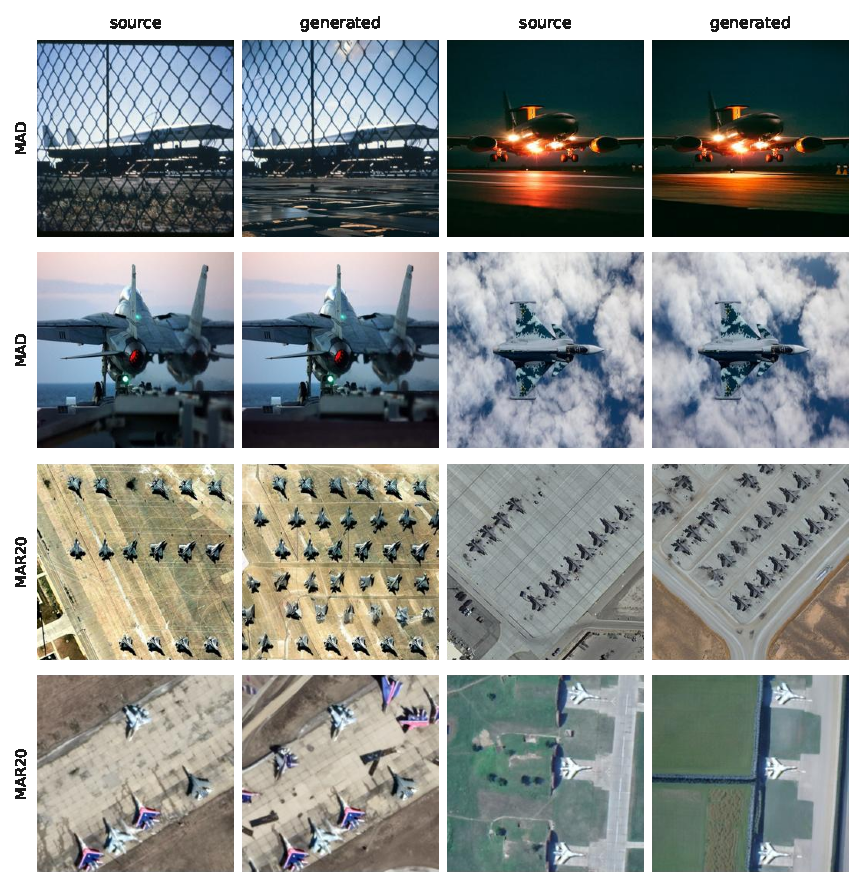
\includegraphics[width=0.92\linewidth]{figures/figa1_gallery.pdf}
\caption{Additional source/generated pairs (backgrounds regenerated;
all annotated objects protected). Top three rows: MAD; bottom row and
right half of row three: MAR20.}
\label{fig:gallery}
\end{figure}

\section{Per-class results}\label{app:perclass}
\begin{table}[h]\centering\small\caption{MAD tail classes: baseline test \mapm{} and per-arm $\Delta$ (3-seed means).}\label{tab:pc-mad-tail}
\begin{tabular}{lrrrrrrr}\toprule
Class & $n$ & base & tail-unif. & tail-prio. & weak-unif. & weak-prio. & RFS \\ \midrule
YF23 & 97 & 0.801 & -0.014 & +0.001 & -0.022 & -0.004 & +0.040 \\
AG600 & 153 & 0.763 & +0.059 & +0.032 & +0.041 & +0.018 & +0.034 \\
Be200 & 209 & 0.757 & +0.020 & +0.012 & +0.023 & -0.003 & +0.078 \\
P3 & 118 & 0.712 & -0.000 & +0.051 & +0.000 & +0.004 & +0.063 \\
XB70 & 119 & 0.656 & +0.041 & +0.077 & +0.055 & +0.014 & +0.103 \\
Mig31 & 225 & 0.636 & +0.101 & +0.101 & -0.006 & -0.010 & +0.132 \\
SR71 & 206 & 0.627 & +0.068 & +0.054 & +0.040 & +0.046 & +0.131 \\
Tu160 & 192 & 0.598 & +0.056 & +0.125 & +0.055 & +0.060 & +0.163 \\
E7 & 86 & 0.592 & +0.060 & +0.065 & +0.001 & +0.036 & +0.045 \\
Su34 & 210 & 0.565 & +0.072 & +0.058 & +0.030 & +0.075 & +0.045 \\
Tu95 & 197 & 0.505 & +0.169 & +0.132 & -0.042 & +0.110 & +0.144 \\
U2 & 208 & 0.439 & +0.084 & +0.088 & -0.015 & +0.009 & +0.106 \\
RQ4 & 212 & 0.404 & +0.062 & +0.010 & +0.027 & +0.030 & +0.194 \\
\bottomrule\end{tabular}\end{table}
\begin{table}[h]\centering\small\caption{MAD weak classes: baseline test \mapm{} and per-arm $\Delta$ (3-seed means).}\label{tab:pc-mad-weak}
\begin{tabular}{lrrrrrrr}\toprule
Class & $n$ & base & tail-unif. & tail-prio. & weak-unif. & weak-prio. & RFS \\ \midrule
Tornado & 273 & 0.561 & +0.047 & +0.048 & +0.123 & +0.096 & +0.106 \\
F4 & 411 & 0.555 & -0.026 & -0.036 & +0.014 & -0.015 & +0.052 \\
F35 & 746 & 0.518 & +0.029 & +0.035 & +0.046 & +0.076 & +0.066 \\
Mirage2000 & 297 & 0.513 & +0.041 & +0.039 & +0.069 & +0.056 & +0.183 \\
F15 & 851 & 0.481 & +0.014 & +0.032 & +0.030 & +0.023 & +0.106 \\
EF2000 & 388 & 0.475 & +0.053 & -0.015 & +0.059 & +0.048 & +0.158 \\
F16 & 902 & 0.468 & +0.048 & +0.028 & +0.070 & +0.046 & +0.095 \\
C17 & 348 & 0.465 & +0.013 & +0.026 & +0.060 & +0.068 & +0.148 \\
F22 & 450 & 0.450 & +0.032 & -0.004 & -0.011 & -0.018 & +0.004 \\
JAS39 & 350 & 0.428 & +0.018 & +0.013 & +0.010 & +0.024 & +0.193 \\
F18 & 885 & 0.416 & +0.022 & +0.013 & +0.042 & +0.024 & +0.091 \\
F14 & 358 & 0.331 & +0.030 & -0.129 & -0.006 & -0.040 & +0.177 \\
Rafale & 369 & 0.269 & +0.078 & +0.039 & +0.086 & +0.048 & +0.137 \\
\bottomrule\end{tabular}\end{table}
\begin{table}[h]\centering\small\caption{MAR20 (all 20 classes): baseline test \mapm{} and per-arm $\Delta$ (3-seed means).}\label{tab:pc-mar20}
\begin{tabular}{lrrrrrrr}\toprule
Class & $n$ & base & tail-unif. & tail-prio. & weak-unif. & weak-prio. & RFS \\ \midrule
A7 & 150 & 0.743 & +0.022 & +0.015 & +0.023 & -0.007 & -0.008 \\
A17 & 360 & 0.738 & -0.008 & +0.005 & -0.017 & -0.017 & +0.005 \\
A10 & 305 & 0.686 & -0.005 & -0.003 & -0.015 & -0.013 & -0.016 \\
A2 & 590 & 0.678 & +0.002 & +0.000 & -0.022 & -0.018 & -0.005 \\
A6 & 84 & 0.673 & +0.016 & +0.028 & +0.011 & -0.002 & +0.029 \\
A8 & 289 & 0.658 & -0.015 & +0.006 & -0.035 & -0.041 & +0.008 \\
A9 & 418 & 0.652 & +0.000 & -0.002 & -0.029 & -0.031 & -0.019 \\
A14 & 536 & 0.647 & +0.003 & +0.012 & -0.011 & -0.007 & +0.004 \\
A4 & 149 & 0.627 & +0.058 & +0.066 & +0.034 & +0.038 & +0.057 \\
A3 & 252 & 0.617 & +0.038 & +0.030 & +0.004 & -0.003 & +0.029 \\
A1 & 441 & 0.605 & -0.046 & -0.062 & -0.014 & -0.017 & -0.017 \\
A12 & 198 & 0.603 & -0.021 & -0.027 & +0.005 & +0.009 & -0.001 \\
A20 & 350 & 0.558 & -0.008 & -0.018 & +0.014 & +0.015 & +0.009 \\
A16 & 648 & 0.524 & +0.047 & +0.057 & +0.074 & +0.077 & -0.010 \\
A11 & 127 & 0.517 & -0.006 & +0.030 & -0.017 & -0.032 & -0.015 \\
A19 & 394 & 0.512 & +0.008 & -0.016 & +0.022 & +0.016 & -0.003 \\
A13 & 463 & 0.426 & +0.005 & -0.016 & +0.008 & +0.016 & +0.006 \\
A18 & 117 & 0.419 & +0.011 & +0.049 & -0.045 & -0.048 & +0.044 \\
A5 & 366 & 0.343 & +0.014 & +0.021 & +0.049 & +0.045 & -0.022 \\
A15 & 165 & 0.214 & +0.079 & +0.072 & +0.044 & +0.073 & -0.011 \\
\bottomrule\end{tabular}\end{table}
\section{Generation quality, hallucination audit, and object-level gate}\label{app:audit}
\paragraph{Quality metrics}
FID (torchmetrics FrechetInceptionDistance, Inception-V3 features) is computed per pool against the real training images containing that pool's target classes, so the reference sets differ across pools and cross-pool FID is indicative rather than strictly comparable; CLIPScore (\texttt{openai/clip-vit-base-patch16}) measures image--prompt similarity and LPIPS (AlexNet backbone) measures source--output distance, both on 200 sampled images per pool. The metrics were computed in the exploratory phase and therefore cover the three originally generated pools; the weak-uniform pool, generated later in the confirmatory phase, passed the same rule-based verification but was not scored.
\begin{table}[h]\centering\small\caption{Per-pool quality metrics (three exploratory-phase MAD pools).}\label{tab:quality}
\begin{tabular}{lrrrr}\toprule
Pool & FID & FID ref.\ ($n$ real) & CLIPScore & LPIPS \\ \midrule
tail-uniform & 89.7 & 1,797 & 19.6 $\pm$ 3.3 & 0.262 \\
tail-priority & 87.7 & 1,797 & 19.1 $\pm$ 3.8 & 0.244 \\
weak-priority & 100.4 & 3,744 & 20.2 $\pm$ 3.4 & 0.272 \\
\bottomrule\end{tabular}\end{table}
A detector-based scan of all 3{,}000 MAD synthetic images (the three originally generated pools) flagged images containing hallucinated, unlabeled aircraft. Table~\ref{tab:gate} reports per-pool removal statistics; a detector-based paired audit of a 450-image sample (150 per pool) flagged a net increase in off-mask detections in 10.2\% of images, consistent with the 11.1\% full-scan removal rate.
\begin{table}[h]\centering\small\caption{Object-level gate: full-corpus scan of the MAD pools.}\label{tab:gate}
\begin{tabular}{lrrrr}\toprule
Pool & images & removed & removed (\%) & flagged objects removed \\ \midrule
tail-priority & 1000 & 82 & 8.2 & 159 \\
tail-uniform & 1000 & 85 & 8.5 & 170 \\
weak-priority & 1000 & 165 & 16.5 & 516 \\
\midrule total & 3000 & 332 & 11.1 & 845 \\
\bottomrule\end{tabular}\end{table}
Retraining the three arms on gated pools (seed matched to the ungated runs) changed macro \mapm{} only marginally:
\begin{table}[h]\centering\small\caption{Gated $-$ ungated macro \mapm{} (single matched seed).}\label{tab:gated}
\begin{tabular}{lrrr}\toprule Arm & all & tail & weak \\ \midrule
tail-uniform & +0.005 & +0.009 & -0.009 \\
tail-priority & -0.017 & -0.012 & -0.021 \\
weak-priority & -0.001 & -0.002 & -0.008 \\
\bottomrule\end{tabular}\end{table}

\begin{figure}[h]\centering
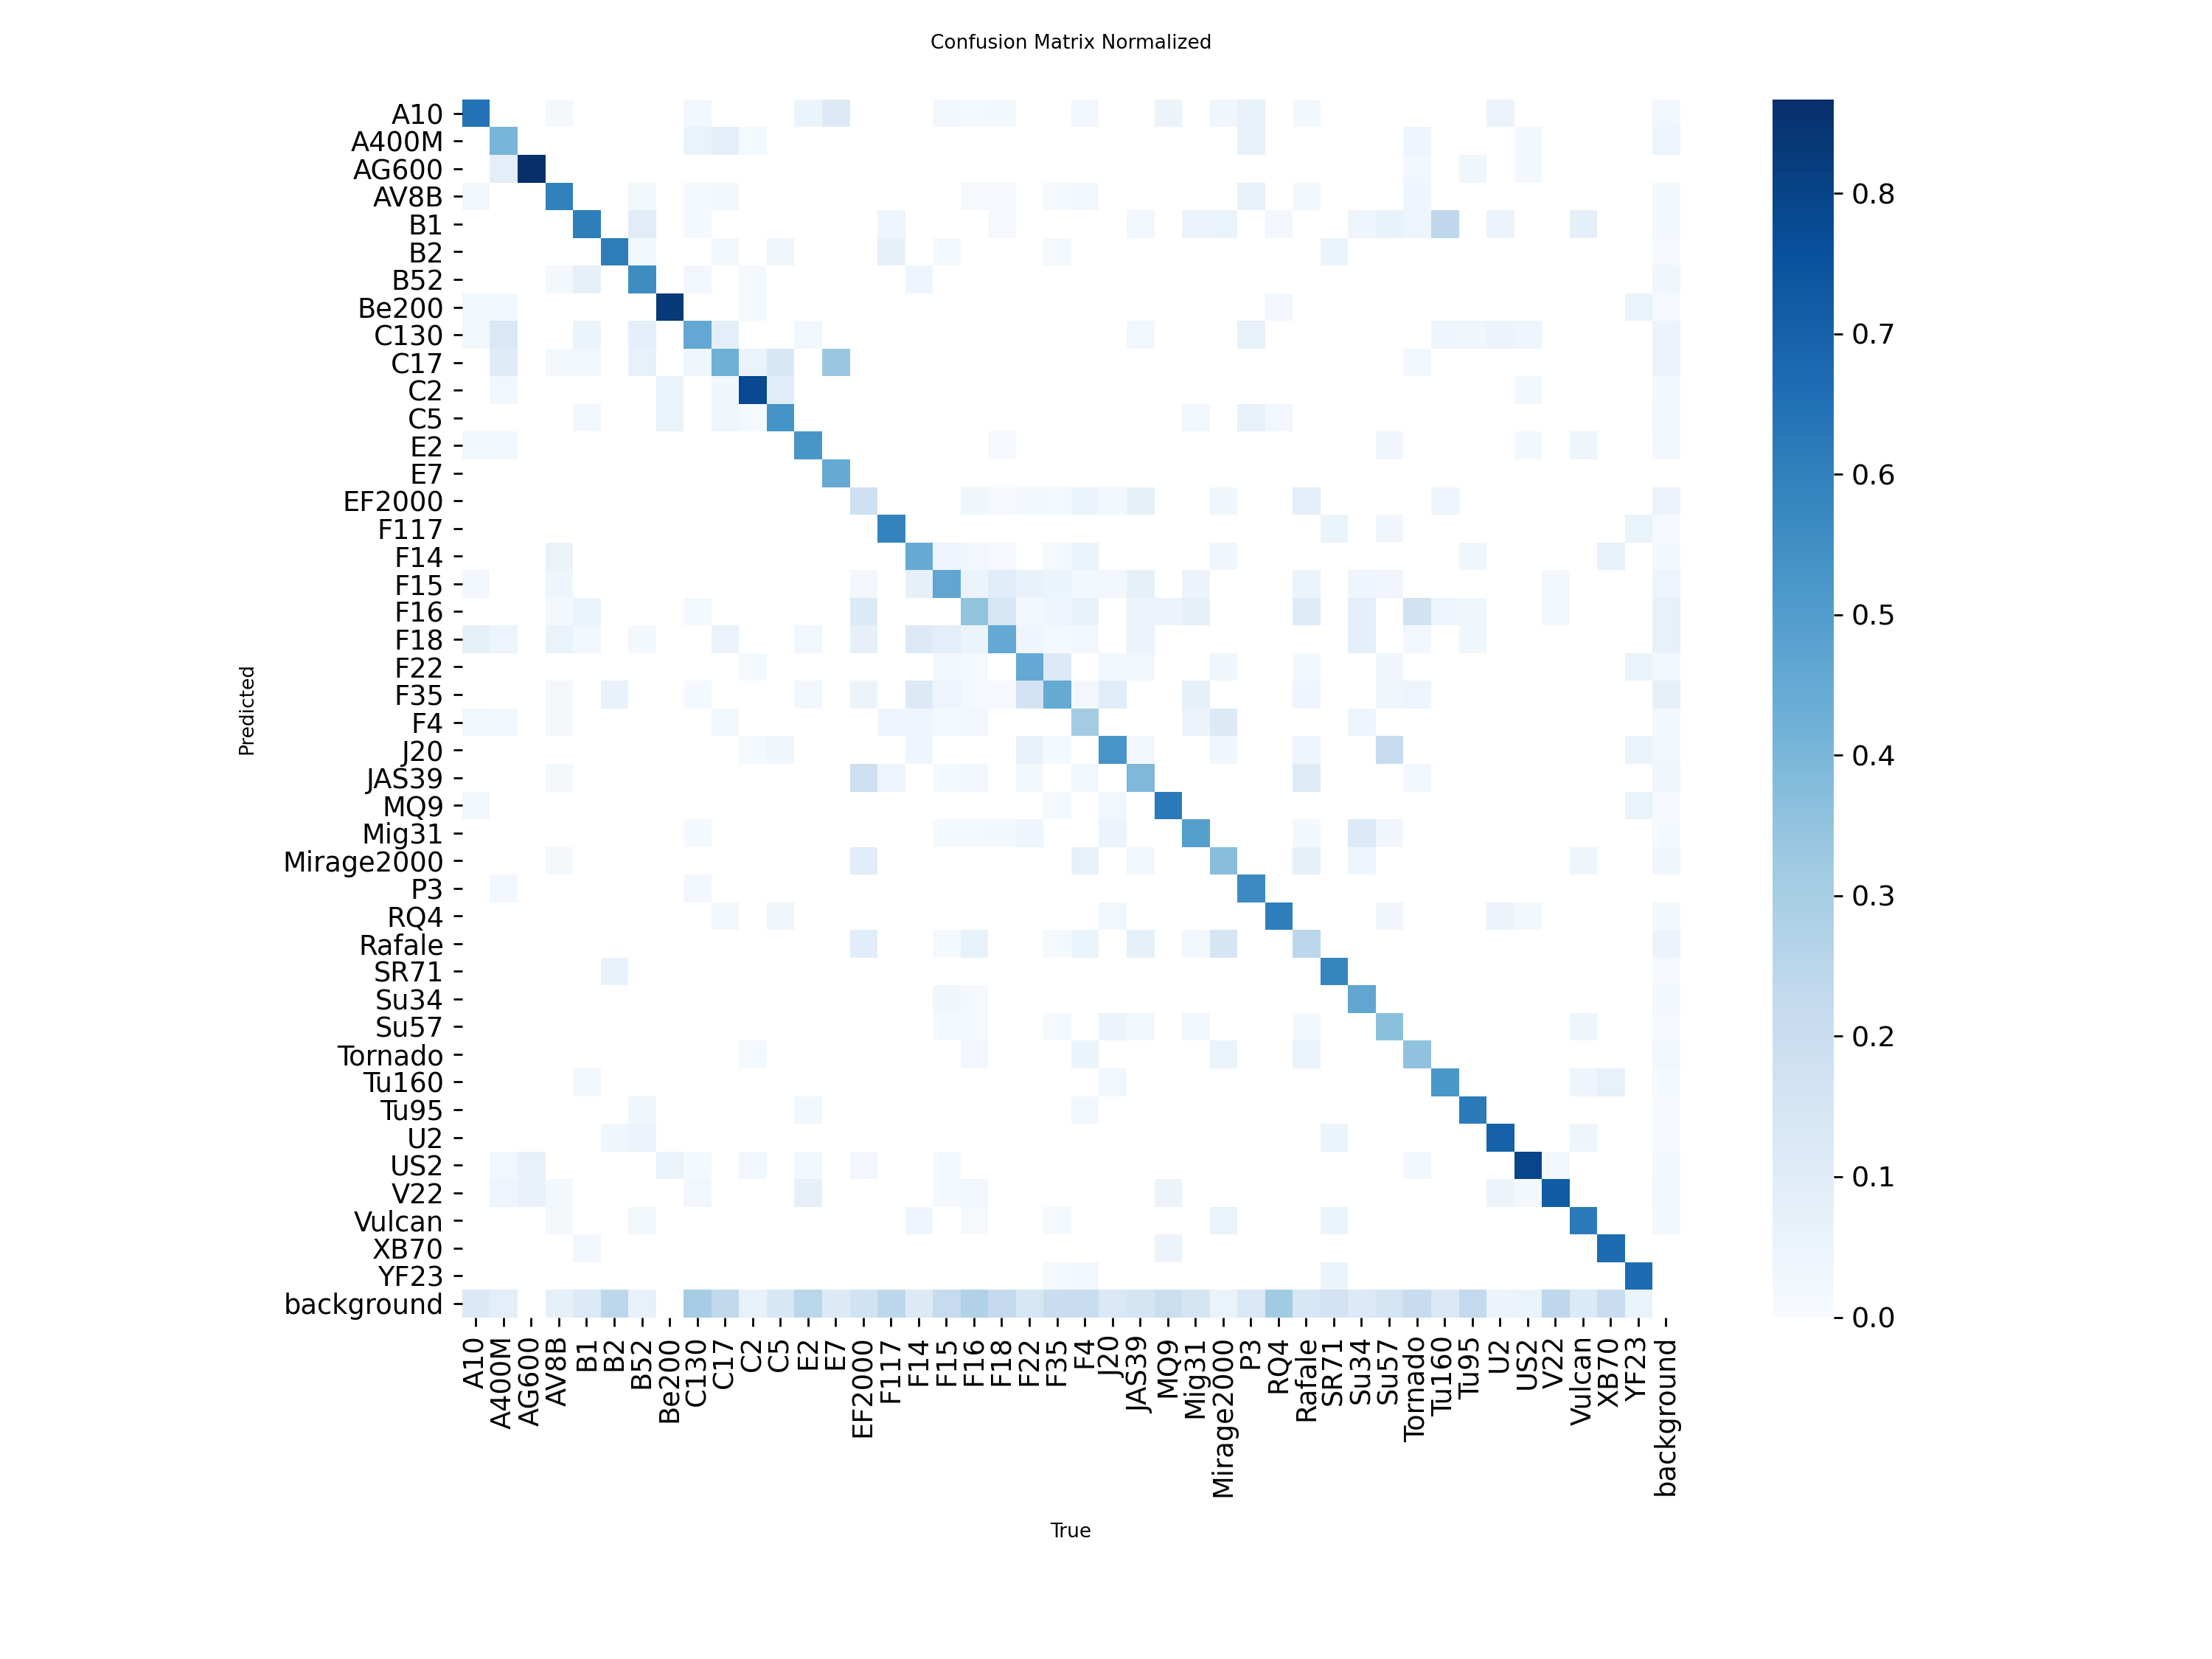
\includegraphics[width=0.9\linewidth]{figures/figa2_confusion.png}
\caption{Normalized confusion matrix of the MAD \texttt{basic\_aug}
baseline (one seed). The dominant off-diagonal mass lies in the
background row (missed detections), the error mode hypothesized to be
affected by background diversification (Section~\ref{sec:mechanism}).}
\label{fig:confusion}
\end{figure}



\bibliographystyle{elsarticle-harv}
\bibliography{refs}

\end{document}
